\documentclass[11pt, a4paper]{article}

\usepackage[left=2cm, text={17cm, 24cm}, top = 3cm]{geometry}
\usepackage{times}
\usepackage[utf8]{inputenc}
\usepackage{verbatim}
\usepackage{amssymb}
\usepackage{multirow}
\usepackage[czech, ruled, noline,  linesnumbered, longend]{algorithm2e}
\usepackage{algpseudocode}
\usepackage[czech]{babel}
\usepackage{graphics}
\usepackage{pdflscape}
\usepackage{hyperref}
\urlstyle{rm}

\begin{document}
\begin{titlepage}
\begin{center}
\Huge
\textsc{Vysoké učení technické v~Brně}\\
\huge
\textsc{Fakulta informačních technologií}\\
\vspace{\stretch{0.382}}
\LARGE Typografie a publikování\,--\,3. projekt\\
\Huge Tabulky a~obrázky
\vspace{\stretch{0.618}}
\end{center}
{\Large 20. března 2018 \hfill
Sabína Gregušová}
\end{titlepage}


\section{Úvodní strana}
Název práce umístěte do zlatého řezu a nezapomeňte uvést dnešní datum a vaše jméno a příjmení.

\section{Tabulky}
Pro sázení tabulek můžeme použít buď prostředí \texttt{tabbing} nebo prostředí \texttt{tabular}.

\subsection{Prostředí \texttt{tabbing}}
Při použití \texttt{tabbing} vypadá tabulka následovně:
\begin{tabbing}
\textbf{Ovoce} \qquad\qquad \= \textbf{Cena} \qquad \= \textbf{Množství}\\
Jablka \> 25,90 \> 3 kg\\
Hrušky \> 27,40 \> 2,5 kg\\
Vodní melouny \> 35,-- \> 1 kus
\end{tabbing}
\bigskip
Toto prostředí sa dá také použíť pro sázení algoritmů, ovšem vhodnejší je použít prostředí \texttt{algorithm} nebo \texttt{algorithm2e }(viz sekce \ref{sec:algoritmy}).

\subsection{Prostředí \texttt{tabular}}
Další možností, jak vytvořit tabulku, je použít prostředí \texttt{tabular}. Tabulky pak budou vypadat takto\footnote{Kdyby byl problem s~\texttt{cline}, zkuste sa podívat třeba sem: \url{http://www.abclinuxu.cz/tex/poradna/show/325037}.}:
\bigskip

\begin{table}[h]
\catcode`\-=12
\begin{center}
\begin{tabular}{| l | r | r |}
\hline
& \multicolumn{2}{| c |}{\textbf{Cena}}\\ \cline{2-3}
\textbf{Měna} & \textbf{nákup} & \textbf{prodej}\\
\hline
EUR & 27,02 & 27,20\\
GBP & 31,08 & 31,80\\
USD & 25,15 & 25,51\\
\hline
\end{tabular}
\caption{Tabulka kurzů k~dnešnímu dni}
\label{tab:kurzy}
\end{center}
\end{table}


\begin{table}[h]
\catcode`\-=12
\begin{center}
\begin{tabular}{| c | c |}
\hline
$A$ & $\neg A$\\ \hline
\textbf{P} & N\\ \hline
\textbf{O} & O\\ \hline
\textbf{X} & X\\ \hline
\textbf{N} & P\\ \hline
\end{tabular}
\begin{tabular}{| c | c | c | c | c | c |}
\hline
\multicolumn{2}{| c |}{\multirow{2}{*}{$ A \wedge B $}} & \multicolumn{4}{c |}{$ B $}\\ \cline{3-6}
\multicolumn{2}{| c |}{} & \textbf{P} & \textbf{O} & \textbf{X} & \textbf{N} \\ \hline
\multirow{4}{*}{$A$} & \textbf{P} & P & O~& X & N \\ \cline{2-6}
& \textbf{O} & O~& O~& N & N \\ \cline{2-6}
& \textbf{X} & X & N & X & N \\ \cline{2-6}
& \textbf{N} & N & N & N & N \\ \cline{2-6}
\hline
\end{tabular}
\begin{tabular}{| c | c | c | c | c | c |}
\hline
\multicolumn{2}{| c |}{\multirow{2}{*}{$A \vee B$}} & \multicolumn{4}{c |}{$ B $} \\ \cline{3-6}
\multicolumn{2}{| c |}{} & \textbf{P} & \textbf{O} & \textbf{X} & \textbf{N} \\ \hline
\multirow{4}{*}{$A$} & \textbf{P} & P & P & P & P \\ \cline{2-6}
& \textbf{O} & P & O~& P & O~\\ \cline{2-6}
& \textbf{X} & P & P & X & X \\ \cline{2-6}
& \textbf{N} & P & O~& X & N \\ \cline{2-6}
\hline
\end{tabular}
\begin{tabular}{| c | c | c | c | c | c |}
\hline
\multicolumn{2}{| c |}{\multirow{2}{*}{$A \rightarrow B$}} & \multicolumn{4}{c |}{$ B $} \\ \cline{3-6}
\multicolumn{2}{| c |}{} & \textbf{P} & \textbf{O} & \textbf{X} & \textbf{N} \\ \hline
\multirow{4}{*}{$A$} & \textbf{P} & P & O~& X & N \\ \cline{2-6}
& \textbf{O} & P & O~& P & O~\\ \cline{2-6}
& \textbf{X} & P & P & X & X \\ \cline{2-6}
& \textbf{N} & P & P & P & P \\ \cline{2-6}
\hline
\end{tabular}
\caption{Protože Kleeneho trojhodnotová logika už je \uv{zastaralá}, uvádíme si zde pŕíklad čtyřhodnotové logiky}
\label{tab:logika}
\end{center}
\end{table}

\section{Algoritmy}
\label{sec:algoritmy}
Pokus budeme chtít vysázet algoritmus, můžeme použít prostředí\texttt{ algorithm}\footnote{Pro nápovědu, jak zacházet s~prostředím \texttt{algorithm,} můžeme zkusit tuhle stránku: \\\url{http://ftp.cstug.cz/pub/tex/CTAN/macros/latex/contrib/algorithms/algorithms.pdf}.}\quad nebo \texttt{algorithm2e}\footnote{Pro\texttt{ algorithm2e} zase tuhle: \url{http://ftp.cstug.cz/pub/tex/CTAN/macros/latex/contrib/algorithm2e/doc/algorithm2e.pdf}.}. Příklad použití prostředí \texttt{algorithm2e }viz Algoritmus \ref{alg:fastslam}.

\begin{algorithm}
\caption{\textsc{FastSLAM}}
\label{alg:fastslam}

\SetNlSkip{-1em}
\SetInd{1em}{1em}
\SetNlSty{}{}{:}
\SetAlgoNlRelativeSize{-1}


\KwIn{$(X_{t-1}, u_t, z_t)$}
\KwOut{$X_t$}
\BlankLine

\Indp \Indpp
$\overline{X_t} = X_t = 0$\\


\For{$k = 1$ \emph{to} $M$}{
$x_t^{[k]} = \emph{sample\_motion\_model}(u_t, x_{t-1}^{[k]})$\\
$\omega_t^{[k]} = \emph{measurement\_model}(z_t, x_t^{[k]}, m_{t-1}^{[k]})$\\
$m_t^{[k]} = \emph{updated\_occupancy\_grid}(z_t, x_t^{[k]}, m_{t-1}^{[k]})$\\
$\overline{X_t} = \overline{X_t} + \langle x_x^{[m]}, \omega_t^{[m]} \rangle $\\}
\For{$k = 1 $ \emph{to} $M$}{
draw $i$ with probability $\approx \omega_t^{[i]}$\\
add $ \langle x_x^{[k]}, m_t^{[k]} \rangle $ to $X_t$}
\Return{$X_t$}
\end{algorithm}

\section{Obrázky}
Do našich článků můžeme samozřejmě vkládat obrázky. Pokud je obrázkem fotografie, můžeme klidně použít bitmapový soubor. Pokud by to ale mělo být nějaké schéma nebo něco podobného, je dobrým zvykem takovýto obrázek vytvořit vektorově.

\begin{figure}[h]
\begin{center}
\scalebox{0.4}{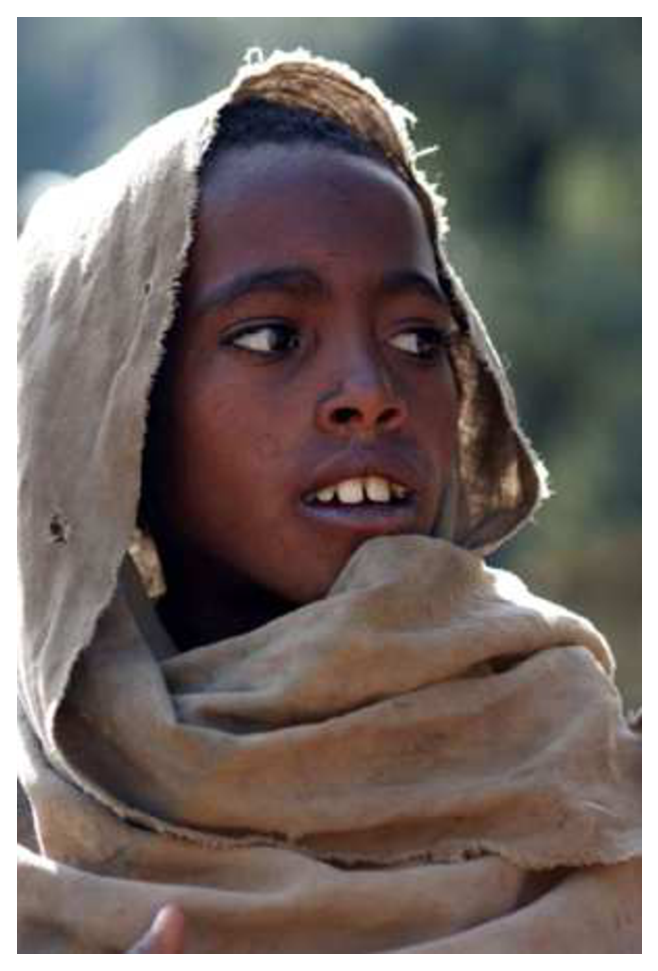
\includegraphics{etiopan.eps}
\reflectbox{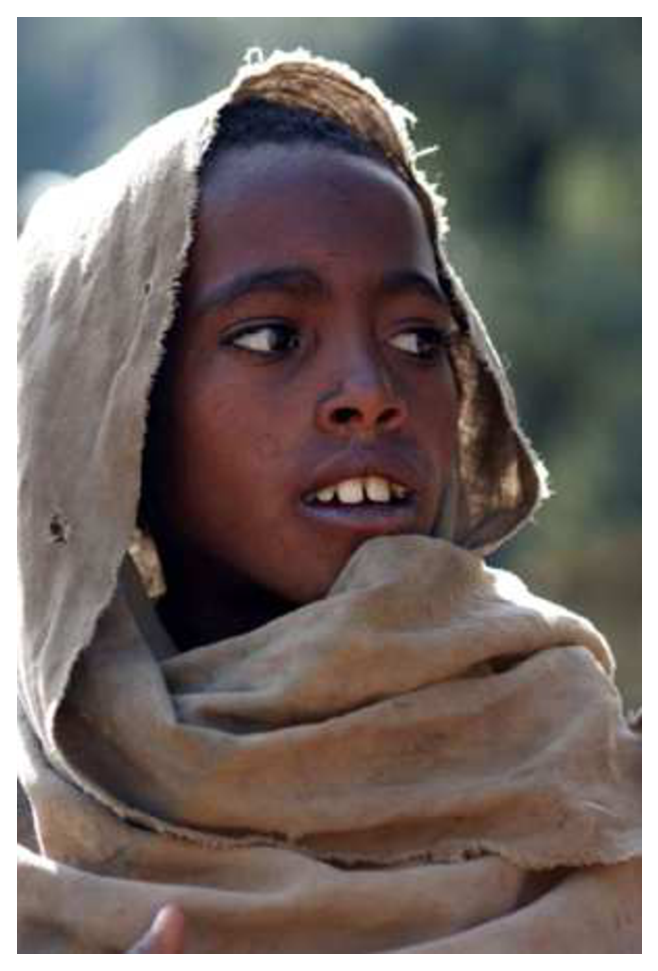
\includegraphics{etiopan.eps}}}
\caption{Malý Etiopánek a jeho bratříček}
\label{fig:Etiopan}
\end{center}
\end{figure}


Rozdíl mezi vektorovým \dots
\begin{figure}[h]
\begin{center}
\scalebox{0.4}{
\includegraphics{oniisan.eps}}
\caption{Vektorový obrázek}
\label{fig:Brat1}
\end{center}
\end{figure}

\dots a bitmapovým obrázkem
\begin{figure}[h]
\begin{center}
\scalebox{0.6}{
\includegraphics{oniisan2.eps}}
\caption{Bitmapový obrázek}
\label{fig:Brat2}
\end{center}
\end{figure}

\noindent
sa projeví například při zvětšení.

Odkazy (nejen ty) na obrázky \ref{fig:Etiopan}, \ref{fig:Brat1} a \ref{fig:Brat2}, na tabulky \ref{tab:kurzy} a \ref{tab:logika} a také na algoritmus \ref{alg:fastslam} jsou udělány pomocí křížových odkazů. Pak je ovšem potřeba zdrojový soubor přeložit dvakrát.

Vektorové obrázky lze vytvořit i přímo v~\LaTeX u, například pomocí prostředí \texttt{ picture}.

\begin{landscape}

\begin{figure}[h]
\begin{center}
\setlength{\unitlength}{1mm}
\begin{picture}(200, 115)
\linethickness{1pt}
\put(0, 0){\framebox(200, 104){}}

% zvislé čiary


\put(115, 45){\line(0, 1){10}}

\put(65, 45){\line(0, 1){10}}
\put(45, 40){\line(0, 1){5}}
\put(25, 15){\line(0, 1){35}}
\put(35, 15){\line(0, 1){15}}
\put(78, 27){\line(0, 1){11}}

\put(165, 45){\line(0, 1){3}}
\put(175, 40){\line(0, 1){5}}
\put(175, 15){\line(0, 1){8}}
\put(173, 23){\line(0, 1){15}}



% vertikálne čiary
\put(35, 30){\line(1, 0){35}}
\put(25, 50){\line(1, 0){40}}
\put(45, 45){\line(1, 0){130}}
\put(45, 40){\line(1, 0){130}}
\put(65, 55){\line(1, 0){50}}
\put(115, 48){\line(1, 0){50}}
\put(91, 23){\line(1, 0){84}}
\put(78, 38){\line(1, 0){95}}

% kruh
\put(165, 85){\circle{16}}

% šikmé čiary
\put(70, 30){\line(3, -1){45}}
\put(45, 40){\line(1, -1){10}}


% hlavná hrubá čiara
{\linethickness{1.6mm}
\put(10, 15){\line(1, 0){180}}}

\end{picture}
\caption{Vektorový obrázok}
\end{center}

\end{figure}


\end{landscape}


\end{document}